\documentclass[12pt]{article}
\usepackage{mathtools,booktabs}
\usepackage[amssymb,cdot]{SIunits}
%\usepackage[utopia]{mathdesign}     
\usepackage[table]{xcolor}
\usepackage{amsmath}
\usepackage{hyperref}
\usepackage{longtable}
\usepackage{fullpage}
\usepackage{listings}
\usepackage{enumitem}
\setlist{nolistsep}

\definecolor{lightgray}{gray}{0.93}

\definecolor{light-gray}{gray}{0.95}
\lstset{basicstyle=\footnotesize\ttfamily,
        %numbers=left,
        %backgroundcolor=\color{light-gray},
        frame=single, 
        %rulesepcolor=\color{red},
        keywordstyle=\color[rgb]{0,0,1},
        commentstyle=\color[rgb]{0.133,0.545,0.133},
        stringstyle=\color[rgb]{0.627,0.126,0.941},
        captionpos=b,
        %title=\lstname,
        showstringspaces=false
       }

\pagestyle{empty}
\setlength\parindent{0pt}
\renewcommand{\thefootnote}{\fnsymbol{footnote}}
 
\makeatletter
\renewcommand\section{\@startsection{section}{1}{\z@}%
                                  {-3.5ex \@plus -1ex \@minus -.2ex}%
                                  {2.3ex \@plus.2ex}%
                                  {\normalfont\bfseries}}
\makeatother


\begin{document}

{\large
  \begin{center}
    {\bf ME 701 -- Development of Computer Applications in ME \\ 
         Homework  5 -- Object-Oriented Python -- Due 10/18/2017 \\
         {\small (Revised: \today)}
    }
  \end{center}

\setlength{\unitlength}{1in}

\begin{picture}(6,.1) 
\put(0,0) {\line(1,0){7.35}}         
\end{picture}
}

{\bf Instructions}.  This homework focuses on the development of a
simple 2-D constructive solid geometry module.  I have provided you
with templates for many of classes you need to define.  The following
problems provide software specifications for pieces of your 
module, starting from points, and building on up through a 
whole geometry made of regions.  \\

To help you in your development,
I've also provide a small unit test framework.
The various {\bf unit tests demonstrate how your classes and methods
should work} for a few cases.  The tests I provide may not provide
complete {\it coverage}, i.e., they might not test every method
for every possible use consistent with the specifications below.
You should feel free to modify these tests and add your own.  
Such testing is extremely helpful for all but the smallest programming
tasks, as it (1) formalizes the normal testing you would do in a (probably) much
sloppier way and (2) lives on as a set of (hopefully) easily understood
examples for how your code works.  Invaluable for the coder with 
the memory of a (dying) goldfish.

\section*{Problem 1 -- On Point}

We started off our discussion of object-oriented programming
using the {\tt Point} class as an example.  In essence, a 
{\tt Point} represents a point in 2-D space (or, equivalently,
a 2-D vector starting from the origin).  In some applications,
it would be helpful to add two points (a translation), or to 
multiply a point by some constant (a scaling), e.g.,

\lstinputlisting[language=Python]{points.py}

{\bf \textcolor{purple}{Deliverables}}: 
modify the basic {\tt Point} class to handle (1) addition of
two points and (2) scaling of a point by a scalar value.  


\section*{Problem 2 -- Nodes and Surfaces}

The template code includes definitions for 
an abstract {\tt Node} class, from which 
the {\tt Primitive} and {\tt Operator} classes 
are derived.  Recall that an abstract class 
is one that defines a method signature but 
does not provide an implementation.  In 
C-speak, it's like having a function declaration
in a header without its definition in
the source file.  A {\it concrete} class inherits
from a {\it base} class and provides an 
implementation of the methods. \\


The {\tt Primitive} class is a concrete class 
that represents
terminal node, i.e., a surface.  On the other hand,
the  {\tt Operator} class represents a generic combination
of two nodes.  Like {\tt Node}, 
{\tt Operator} is an abstract
class because its {\tt contains} method is 
not (and should not) be implemented.  Its other 
method {\tt intersections}   should be defined,
however, and that's for you to do. \\

In addition,  you  
should create the following two specializations
of the {\tt Operator} class:
\begin{itemize}
 \item {\tt class Union}, whose method {\tt contains(p)}
       should return true if the point is in either 
       its left or right nodes.
 \item {\tt class Intersection}, whose {\tt contains(p)}
       should return true if the point is in both 
       its left and right nodes.
\end{itemize}

\vspace{12pt}
{\bf \textcolor{purple}{Deliverables}}:
\begin{enumerate}
 \item Implement {\tt Operator.intersections(r)}
 \item Define {\tt class Union} and implement {\tt Union.contains(p)}
 \item Define {\tt class Intersection} and implement {\tt Intersection.contains(p)} 
\end{enumerate}


\section*{Problem 3 -- Kids Love Shapes}

The template code provides partial definitions for 
the abstract {\tt Surface} and concrete 
{\tt QuadraticSurface} classes.  Your
first task is to implement the {\tt f} and {\tt intersections}
methods of {\tt QuadraticSurface}.\\


Although you can define any 2-D quadratic surface with the approach
outlined in the notes, it is easier to specialize that
class further for common cases.  Your job is to 
create the following classes that inherit from {\tt QuadraticSurface}:
\begin{itemize} % Dx + Ey + F = 0,  y = -D - Dx
  \item {\tt class PlaneV}; defines a vertical plane at $x=a$ via
        {\tt v = PlaneV(a)},
  \item {\tt class PlaneH}; defines a horizontal plane at $y=b$ via
        {\tt h = PlaneH(b)}
  \item {\tt class Plane}; defines a plane of the form $y = mx + b$
        via {\tt p = Plane(m, b)}.
  \item {\tt class Circle}; defines a circle of radius $r$ and center $(a, b)$
       via {\tt c = Circle(r, a, b)}.
\end{itemize}
\vspace{12pt}
You could also specialize the methods {\tt intersections}
and {\tt f}, but your implementation of these methods in 
{\tt QuadraticSurface} should work for {\it any} surface 
with the generic form given in the notes, i.e., 
$f(x, y) = Ax^2 + By^2 + Cxy + Dx + Ey + F$. \\

{\bf \textcolor{purple}{Deliverables}}:
\begin{itemize}
 \item Implement {\tt QuadraticSurface.f(p)}
 \item Implement {\tt QuadraticSurface.intersections(r)}
 \item Implement {\tt PlaneV}
 \item Implement {\tt PlaneH}
 \item Implement {\tt Plane}
 \item Implement {\tt Circle}
\end{itemize}


\section*{Problem 4 -- Regions and Geometry}

Now you have surfaces and nodes with which to 
implement a {\tt Region} class.  I've proposed the 
following definition:

\lstinputlisting[language=Python]{region.py}

Study the {\tt append} method because it represents
how we put all the surfaces and nodes together.  The 
key point is that {\tt Region} has an attribute 
{\tt node} that represents at all times the top of 
the tree of nodes and surfaces.  You should add 
an appropriate docstring to explain what the method
is doing, what the assertions are doing, etc.  In 
other words, make it obvious that you know what
I'm doing.  (This might seem like a silly exercise,
but the ability to digest and then add to code
that someone else wrote is a good way to improve
your own programming.) \\

Once you've done that, you need to implement the 
{\tt contains} and {\tt intersections} methods.
In particular, the points returned by the latter
should satisfy the following:
\begin{itemize}
 \item They are unique (a ray might intersect more
       than one surface that defines a region, e.g,
       if the ray is along the $x$-axis and the 
       region is bounded by the planes $y = \pm x$,
       then the point $(0, 0)$ could be included
       twice.)
 \item They include points only along forward of
       the ray origin. For example, if a region
       is bounded by the unit circle centered
       at the origin, then a ray centered at the 
       origin in the positive $x$ direction 
       would intersect the region at  $(1,0)$
       but not $(-1, 0)$.
 \item They are ordered by increasing distance
       from the ray's origin, i.e., the first 
       point is the first one encountered by
       the ray.
\end{itemize}
\vspace{12pt}

Finally, consider the following {\tt Geometry} class:

\lstinputlisting[language=Python]{geometry.py}

Its construction requires a bounding box defined 
by minimum and maximum values for $x$ and $y$, i.e.,
the square domain in which the geometry is confined.
Regions are stored in an initially empty list.  Regions
are added by the {\tt add\_region} method.  Your job
is to implement the {\tt find\_region} method, which 
returns the index (in the list) of the region that
contains the point.  If no region contains the point,
or if the point lives outside the bounding box, return
{\tt Geometry.noregion}. \\

{\bf \textcolor{purple}{Deliverables}}:
\begin{enumerate}
 \item Document {\tt Region.append}  
 \item Implement {\tt Region.contains}
 \item Implement {\tt Region.intersections}
 \item Implement {\tt Geometry.find\_region}
\end{enumerate}

\section*{Bonus Problem -- Challenge!}

I'll give you 2 (actual) bonus points
if you solve it (and 1 for a very valiant effort 
if not successful).\\

Consider a surface formed by wrapping a sine wave around a circle
back onto itself.  We can do so using a parametric curve of the 
form 
\begin{equation}
\begin{split}
  x &= [r+a\sin(n\phi+\phi_0)]\cos(\phi) + x_0 \\
  y &= [r+a\sin(n\phi+\phi_0)]\sin(\phi) + y_0
\end{split}
\end{equation}
where $\phi$ is the parameter, $r$ is the radius of the circle about 
which the wave is wrapped, $a$ is the magnitude of that wave, 
and $(x_0, y_0)$ is the center of the curve. The figure shows 
the resulting curve for
$r=2$, $n = 4$, $a = 0.5$, and $\phi_0 = \pi/2$.

\begin{figure}[h]
 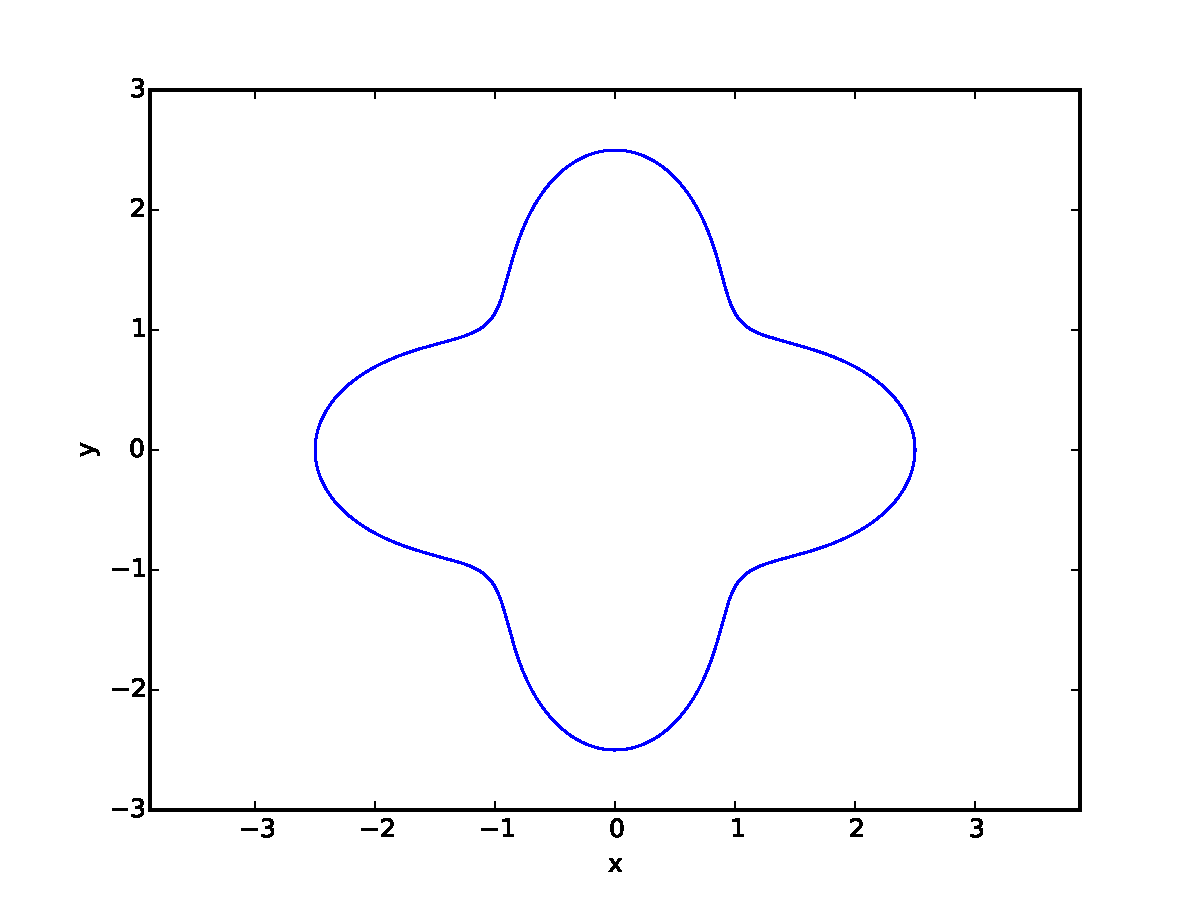
\includegraphics[width=0.5\textwidth]{nonlinear}
\end{figure}

You can convert this into implicit form by moving the $x_0$ and $y_0$
terms to the left side, squaring both equations, and adding the results, which
all leads to 
\begin{equation}
  (x-x_0)^2 + (y-y_0)^2 = [r+a\sin(n\phi+\phi_0)]^2
\end{equation}
or 
\begin{equation}
 f(x, y) = (x-x_0)^2 + (y-y_0)^2 - [r+a\sin(n\phi+\phi_0)]^2 \, .
\end{equation}
That pesky $\phi$ can be found from the original equations by 
noting
\begin{equation}
 \phi = \arctan [(y-y_0)/(x-x_0)] \, .
\end{equation}



{\bf \textcolor{purple}{Deliverables}}:
\begin{enumerate}
 \item Explain how you would tackle the intersections problem 
       for this surface.
 \item Do it!
\end{enumerate}





\end{document}